\documentclass[12pt, letterpaper, twoside]{article}

% Load packages
\usepackage{amsmath}      % Advanced math typesetting
\usepackage{graphicx}     % Include graphics
\usepackage{hyperref}     % Hyperlinks

% Metadata
\title{MATH 628 FINAL PROJECT\\PCA Analysis}
\author{Chunlin Shi\\Noah Collins}
\date{\today}

\begin{document}
    \maketitle

    \begin{abstract}
        In this project, we found 1-year daily trading 
        data for the following stocks: AAL, AMD, 
        AVGO, BAC, BRK-A, CVX, DAL, EOG, INTC, JPM, 
        LUV, NVDA, SLB, UAL, WFC, XOM. 
        We repeated the analysis of 
        Sections 2.1-2.2 of the paper by 
        Avellaneda and Lee. 
        We then discussed the signs of the second 
        and the third eigenvectors partition stocks 
        into stocks and discovered that stocks in the 
        same group have the same sign on the second 
        and third eigenvectors, which corresponds to 
        the grouping of the stocks by industries. 
    \end{abstract}

    \section{Introduction}
    Principal Component Analysis is a powerful statistical 
    tool that allows us to explore multidimensional 
    relationships within datasets. 
    In our paper's case, our dataset was 15 stocks 
    and their trading information over a year. 
    PCA analysis helps capture the most significant 
    sources of variation, which in the case of stocks, 
    unveils patterns and correlations that may not be 
    apparent to the naked eye. We seek to delineate groups
    of stocks that share common trends, behaviors, or 
    underlying factors and to compare these results with 
    official industry groupings to demonstrate the 
    efficacy of PCA as a tool for financial 
    professionals, researchers and investors.

    \section{Methodology}
    To conduct this research, 
    we gathered data from the website of Center for 
    Research in Security Prices (CRSP) of 
    Wharton Research Data Services. 
    The time range of the daily trading data is 
    from December 31, 2021, to December 30, 2022. 
    We collected following variables for our study:

    \begin{itemize}
        \item \textbf{Date:}  Date of trading.
        \item \textbf{Ticker Symbol:} Ticker for stocks accordingly.
        \item \textbf{North American Industry Classification System:} 
        Code used to proxy belonging industry of the stock.
        \item \textbf{Price or Bid/Ask Average, Shares Outstanding:} 
        Variables used to construct market cap weighted 
        portfolios.
        \item \textbf{Returns without Dividends:} 
        Daily return data used for 
        PCA analysis and eigen portfolio construction..
    \end{itemize}
    
    \section{Implementation of the Analysis in the Paper by Avellaneda and Lee}
    \subsection{Section 2.2}
    According to the Paper, the daily return is calculated by:
    $$R_{ik}=\frac{S_{i(t_0-(k-1)\Delta t)}-
    S_{i(t_0-k\Delta t)}}{S_{i(t_0-k\Delta t)}}, 
    k=1, \cdots, M, i=1, \cdots, N $$
    Where $M=252$ and $N=16$, and $S_{it}$ is the price of 
    stock $i$ at time $t$ adjusted for dividends and 
    $\Delta t=\frac{1}{252}$\\\\
    The return was standardized as follows:
    $$Y_{ik} = \frac{R_{ik}-\overline{R_i} }{\overline{\sigma _i}}$$
    Where,
    $$\overline{R_i}=\frac{1}{M}\sum_{k = 1}^{M} R_{ik} $$

    In our procedures, we used daily return adjusted for 
    dividends from CRSP and used \textit{StandardScalar} in 
    \textit{sklearn} in Python to calculate standardized 
    return matrix. Then, we applied PCA analysis 
    with 3 principal components on the standardized 
    return matrix. We also calculated the correlation 
    matrix based on the standardized return matrix, 
    and generated eigenvalues and plotted them 
    from the largest value to the lowest value. 
    Below is the graph we plot and the graph in the paper:\\
    \begin{figure}[h]
        \centering
        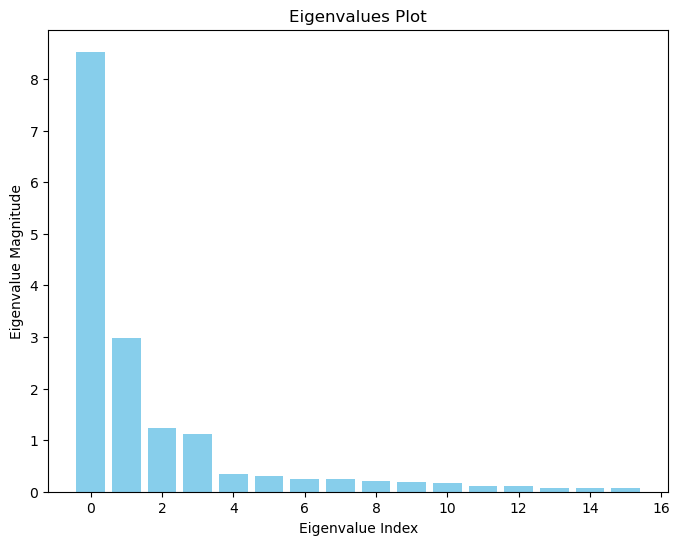
\includegraphics[width=0.8\linewidth]{eigenvalues.png}
        \caption{Plot of eigenvalues}
    \end{figure}
    \begin{figure}[h]
        \centering
        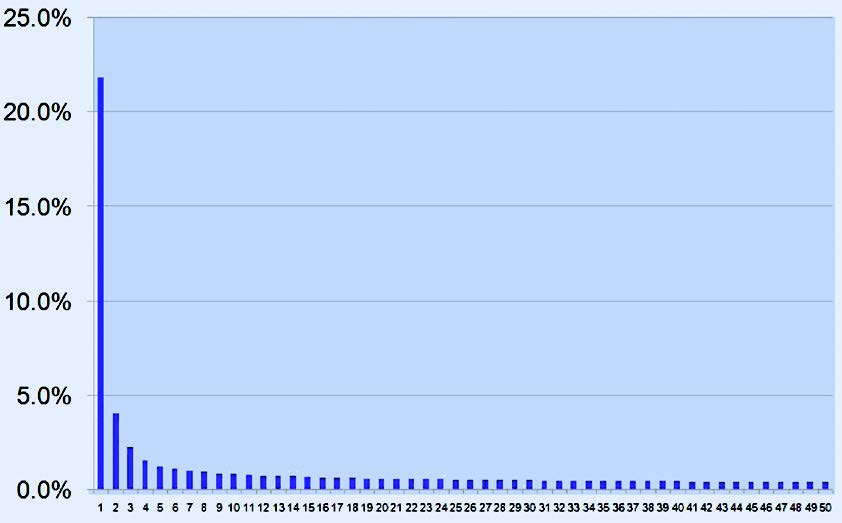
\includegraphics[width=0.8\linewidth]{paper1.jpg}
        \caption{Plot of eigenvalues from \textit{Avellaneda's} paper}
    \end{figure}
    From graphs above, we can see that both graphs show 
    a decreasing trend of the magnitude of eigenvalues.\\\\
    We later conducted a cursory analysis on eigenvalues. 
    Below is the graph we plot and the graph in the paper:
    \begin{figure}[h]
        \centering
        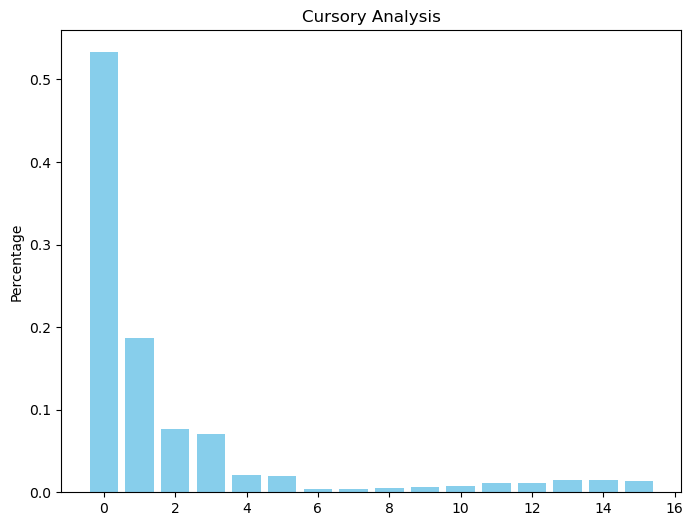
\includegraphics[width=0.8\linewidth]{cursory.png}
        \caption{Cursory analysis}
    \end{figure}
    \begin{figure}[h]
        \centering
        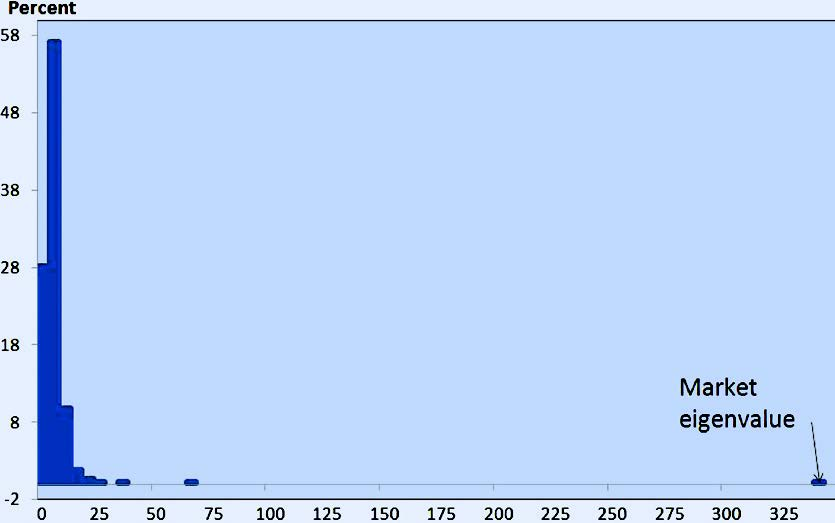
\includegraphics[width=0.8\linewidth]{paper2.jpg}
        \caption{Cursory analysis from \textit{Avellaneda's} paper}
    \end{figure}

    \subsection{Section 2.3}
    In this section, we constructed the eigen portfolio 
    and the market cap weighted portfolio to calculate 
    their cumulative returns. 
    Below is the cumulative return graph we plot 
    and the graph in the paper:
    \begin{figure}[h]
        \centering
        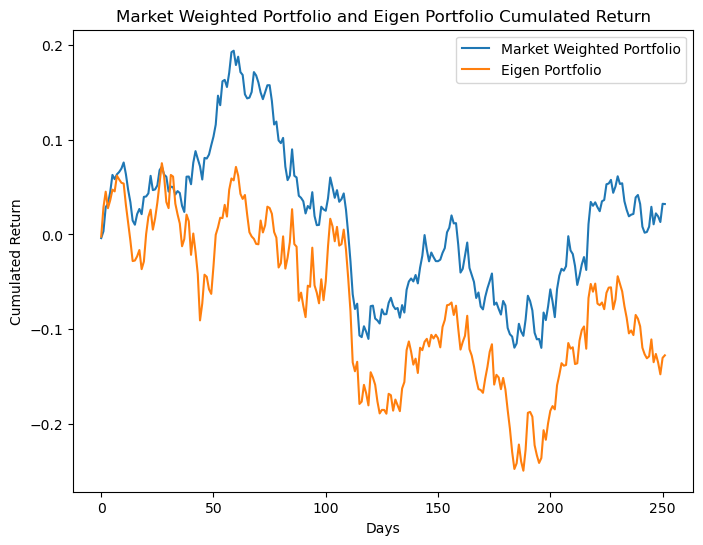
\includegraphics[width=0.8\linewidth]{eigenportfolio.png}
        \caption{Market weighted return and 
        eigenportfolio cumulative return}
    \end{figure}

    \begin{figure}[h]
        \centering
        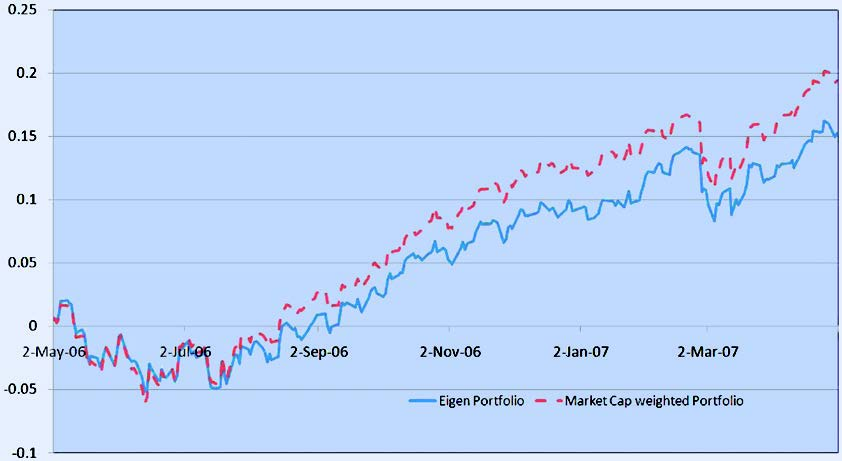
\includegraphics[width=0.8\linewidth]{paper3.jpg}
        \caption{Market weighted return and 
        eigenportfolio cumulative return from \textit{Avellaneda's} paper}
    \end{figure}

    We discovered that our graph showed high similarity 
    with graph provided in the paper that both portfolios 
    showed a comparative evolution, and the cumulative 
    return of the eigen portfolio is slightly lower than 
    market cap weighted portfolio. Hence, this result 
    matches the view in the paper that two portfolios 
    are not identical but are good proxies for each other.
    
    \subsection{The relationship between 
    Signs of the Second and Third Eigenvectors 
    and the Belonging Industry of the Stock}

    In this section, we used the result of PCA analysis 
    with 3 principal components on the standardized 
    return matrix. 

    
    \section{Conclusion}
    Through replication of the original results using 
    a smaller dataset, our project aimed to 
    validate the robustness and generalizability 
    of the findings to a more constrained context. 
    Despite the scale reduction, our results closely 
    mirror those reported in the original paper, 
    demonstrating the consistency of PCA and its 
    ability to group stocks in a matter that 
    corresponds to industries.

    \section*{References}
    \begin{enumerate}
        \item Marco Avellaneda \& Jeong-Hyun Lee (2010) Statistical arbitrage in the US equities market, Quantitative Finance, 10:7, 761-782, DOI: 10.1080/14697680903124632
        \item Wharton Research Data Services. (2022). Wharton Financial Data Services. Retrieved from https://wrds-www.wharton.upenn.edu/
        \item Pandas Development Team. (2023). pandas (1.3.3). Retrieved from https://pandas.pydata.org/
        \item NumPy Community. (2023). NumPy (1.21.2). Retrieved from https://numpy.org/
        \item Matplotlib Development Team. (2023). Matplotlib (3.4.3). Retrieved from https://matplotlib.org/
        \item Scikit-learn Developers. (2023). scikit-learn (0.24.2). Retrieved from https://scikit-learn.org/
    \end{enumerate}

\end{document}
